\documentclass[conference]{IEEEtran}
\usepackage{graphicx,booktabs,amsmath,cite}
\begin{document}
\title{Neighbourhood-Aware Misbehavior Detection in V2X Networks\\ with Cross-Vehicle Attention}
\author{\IEEEauthorblockN{Shlok \quad Caleb \quad Jiya}
\IEEEauthorblockA{School of AI \& Future Technologies}}
\maketitle

\begin{abstract}
Vehicles in V2X networks broadcast Basic Safety Messages (BSMs) roughly ten times per second, and neighbours act on them for safety-critical decisions. Signatures authenticate the sender but not the content, so a credentialed vehicle can still lie about its position. Learned detectors typically score each sender against its own history, which cannot expose the \emph{constant position offset} attack: a fixed displacement preserves speed, acceleration, heading and trajectory shape. We change the model's input rather than its architecture: a transformer encoder attends across co-located senders at the same instant as well as across time, so a claimed position is judged against positions claimed by surrounding vehicles. On a VeReMi-style highway simulator with held-out senders, a per-sender model reaches F1 0.00 on constant position offset, while the neighbourhood-aware model reaches 0.91 and outperforms the identical model with the spatial attention axis disabled (0.82 F1; 0.82 vs.\ 0.76 macro F1). The advantage is not uniform: the per-sender model is better on attacks that break internal consistency. Domain-adversarial transfer to a differently configured traffic scenario gave no reliable gain. \emph{Results here are on simulated data; evaluation on the real VeReMi family is pending.}
\end{abstract}
\begin{IEEEkeywords}
V2X, misbehavior detection, neighbourhood awareness, transformer, cross-vehicle attention, VeReMi, constant position offset.
\end{IEEEkeywords}

\section{Introduction}
V2X safety applications trust the content of BSMs. Certificate infrastructure such as IEEE 1609.2 validates and revokes credentials~\cite{devincenzi}, but cannot establish that a signed position is true, hence learned misbehavior detection is needed alongside it~\cite{abdelhakeem,huang}. Existing learned detectors model each sender independently. This works against attacks that break a sender's internal consistency, but fails on the constant position offset attack: adding a fixed vector to every reported position leaves kinematics unchanged, so the falsified trajectory is indistinguishable from benign mobility under a per-sender view. The strongest published detector is reported to reach F1 of 0.19 on this attack while reaching up to 0.95 on most other categories of the 19 attack types in the benchmark.

We contribute (i) a factorised transformer whose attention runs over time \emph{and} over the variable set of senders heard by a receiver at the same instant, extending cross-vehicle attention, previously demonstrated for coordinated platoons~\cite{attentionguard,attentioninmotion}, to uncoordinated open traffic; (ii) an ablation that removes only the spatial axis, isolating its effect from that of supervision; (iii) a domain-adversarial transfer test; and (iv) open code and an evaluation harness.

\section{Related Work}
Surveys cover machine-learning, federated-learning and edge-AI intrusion detection for V2X~\cite{abdelhakeem} and V2X security and privacy~\cite{huang}. Trust and edge-security designs include a lightweight edge security model~\cite{zhou}, HFLD~\cite{hfld} and PoAh~2.0~\cite{poah}; the latter is a theoretical proposal whose empirical validation is left to future work. None targets learned detection of falsified position content. The VeReMi datasets~\cite{veremi,veremiext,vereming} provide comparable evaluation; AttentionGuard~\cite{attentionguard}, its follow-up~\cite{attentioninmotion} and PAMPOS~\cite{pampos} apply transformers to misbehavior detection.

\section{Method}
\textbf{Receiver-centric samples.} For receiver $r$ and time $t$, we take the $K{=}16$ senders heard at $t$ nearest to $r$ by \emph{claimed} distance, with $T{=}10$ one-second steps of history. Each token $(j,\tau)$ has 8 features: claimed position relative to $r$ (scaled by radio range), speed, $\cos/\sin$ heading, claimed displacement since $\tau{-}1$, and a validity flag. The neighbour set is variable and padded with masking.

\textbf{Model.} Each of $L{=}2$ blocks (width 64, 4 heads) applies temporal self-attention within each sender, then spatial self-attention across senders at each step, then a feed-forward layer. The newest-step representation of each sender goes to an MLP head giving $P(\text{misbehaving})$. In the \emph{no-neighbourhood} ablation the spatial attention mask is the identity, so inputs and parameters are unchanged but no information flows between senders. A \emph{per-sender} baseline additionally zeroes the claimed position features, leaving only each sender's own motion. For transfer, a domain classifier is attached through a gradient-reversal layer~(DANN) with weight $\lambda$.

\textbf{Training.} AdamW, one-cycle LR (peak $2\times10^{-3}$), 5 epochs, batch 128, binary cross-entropy (pos.\ weight 2). The threshold maximises overall F1 on validation data. Per-attack F1 treats that attack's senders as positives and all benign senders as negatives.

\section{Experimental Setup}
\textbf{Data.} We use a VeReMi-style simulator we wrote: a 3-km two-direction, three-lane-per-direction IDM highway loop, 1~Hz BSMs, 300~m radio range, 25\% attackers, 1~m GPS noise. Attackers perform one of five attacks: ConstPos, ConstPosOffset (random fixed offset of 30--120~m), RandPos, RandPosOffset, EventualStop. Train/validation/test sets come from distinct simulation runs with disjoint sender identities (4/1/2 runs; 12.3k/3.1k/6.2k samples). The transfer target is a denser, slower, shorter scenario (2 lanes/direction, 45~veh/km/lane, 250~m range, 1.5~m noise), with unlabeled target data used for DANN and a threshold taken from source validation only. Each configuration is run with 3 seeds (2 for DANN).

\section{Results}
\begin{table}[t]\centering\caption{Per-attack F1 (mean$\pm$std over 3 seeds), held-out senders.}\label{tab:main}\small
\resizebox{\columnwidth}{!}{\begin{tabular}{lcccccc}\toprule
Model & ConstPos & ConstPosOff. & RandPos & RandPosOff. & EvStop & Macro \\\midrule
Per-sender & 0.96$\pm$0.00 & 0.00$\pm$0.00 & 0.98$\pm$0.00 & 0.99$\pm$0.00 & 0.44$\pm$0.00 & 0.68$\pm$0.00 \\
Ours w/o neighbourhood & 0.78$\pm$0.11 & 0.82$\pm$0.05 & 0.94$\pm$0.03 & 0.88$\pm$0.07 & 0.37$\pm$0.04 & 0.76$\pm$0.06 \\
Ours (neighbourhood-aware) & 0.88$\pm$0.02 & 0.91$\pm$0.01 & 0.97$\pm$0.01 & 0.94$\pm$0.01 & 0.41$\pm$0.01 & 0.82$\pm$0.01 \\
\bottomrule\end{tabular}}\end{table}
\begin{table}[t]\centering\caption{Highway$\to$dense transfer (target labels never used). Threshold fixed on source validation.}\label{tab:dann}\small
\begin{tabular}{lcccc}\toprule Training & Macro F1 & Macro AUC & ConstPosOff. F1 & ConstPosOff. AUC\\\midrule
Source only & 0.24$\pm$0.13 & 0.87$\pm$0.01 & 0.30$\pm$0.16 & 0.91$\pm$0.02 \\
DANN $\lambda$=0.05 & 0.27$\pm$0.18 & 0.73$\pm$0.04 & 0.20$\pm$0.09 & 0.63$\pm$0.14 \\
DANN $\lambda$=0.2 & 0.25$\pm$0.17 & 0.83$\pm$0.03 & 0.10$\pm$0.01 & 0.86$\pm$0.06 \\
\bottomrule\end{tabular}\end{table}
\begin{figure}[t]\centering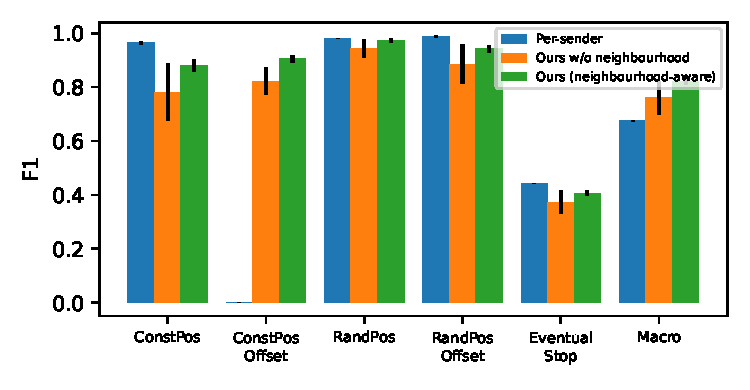
\includegraphics[width=\columnwidth]{fig_perattack.pdf}\caption{Per-attack F1, held-out senders.}\end{figure}

\textbf{Constant position offset.} The per-sender model fails completely (F1 0.00), confirming that this attack is invisible to a sender-only view. The neighbourhood-aware model reaches $0.91\pm0.01$, versus $0.82\pm0.05$ for the same network with the spatial axis disabled (Table~\ref{tab:main}); the ablation shows that cross-sender attention, not merely access to receiver-relative coordinates, contributes the gain. Macro F1 is $0.82\pm0.01$ vs.\ $0.76\pm0.06$.

\textbf{Not uniformly better.} The per-sender model is stronger on ConstPos (0.96), RandPos (0.98) and RandPosOffset (0.99), where jumps or inconsistent motion are visible within one sender's history, and the full model trails it by 0.02--0.08 there. Its lower macro F1 (0.68) is driven by the offset attack and EventualStop. All models are weak on EventualStop (0.37--0.44).

\textbf{Transfer.} Source-only transfer retains ranking quality (macro AUC $0.87$) but F1 collapses ($0.24\pm0.13$) because the source-chosen threshold no longer fits. DANN did not help: macro F1 was within noise ($0.27\pm0.18$, $0.25\pm0.17$) and AUC fell (0.73, 0.83). Variance across two seeds is very large, so we draw no conclusion beyond ``no reliable benefit in this setup.''

\section{Threats to Validity}
\textbf{All results are on simulated data}, produced by a simulator we wrote, not on VeReMi, VeReMi Extension or VeReMi NextGen; the absolute numbers, and the size of the neighbourhood advantage, may not carry over. The simulator's offsets can place a vehicle off-road or in the wrong lane, which a neighbour-aware model can exploit; real VeReMi offsets differ. Our loader for real VeReMi logs is written to the published format but is untested on the real archives. The comparison to the published F1 of 0.19 is therefore not like-for-like. Further, the no-neighbourhood ablation still sees receiver-relative coordinates, so it is not a pure per-sender detector (that role is the per-sender baseline). Seeds are few (3, and 2 for DANN), and the F1 threshold is tuned on validation data.

\section{Conclusion and Future Work}
On simulated traffic, cross-vehicle attention restores detection of the constant position offset attack that a per-sender view cannot see, at some cost on attacks that per-sender models already handle. Next steps: run on real VeReMi and VeReMi Extension/NextGen with held-out sender splits, compare against published detectors, retune the transfer experiments, and release weights and the evaluation harness.

\begin{thebibliography}{99}
\bibitem{abdelhakeem} S. A. Abdel Hakeem and H. Kim, ``Advancing intrusion detection in V2X networks: A comprehensive survey on machine learning, federated learning, and edge AI for V2X security,'' \emph{IEEE Trans. Intell. Transp. Syst.}, vol. 26, no. 8, pp. 11137--11205, 2025.
\bibitem{huang} J. Huang, D. Fang, Y. Qian, and R. Q. Hu, ``Recent advances and challenges in security and privacy for V2X communications,'' \emph{IEEE Open J. Veh. Technol.}, vol. 1, pp. 244--266, 2020.
\bibitem{devincenzi} M. De Vincenzi \emph{et al.}, ``Security risks and designs in the connected vehicle ecosystem: In-vehicle and edge platforms,'' \emph{IEEE Open J. Veh. Technol.}, vol. 6, pp. 442--454, 2025.
\bibitem{zhou} X. Zhou, X. Han, S. Wang, and M. Zhang, ``Lightweight security protection system design for complex V2X scenarios,'' in \emph{Proc. ISEAE}, 2025, pp. 1067--1071.
\bibitem{hfld} S. Fang \emph{et al.}, ``HFLD: A secure and scalable hybrid framework for intelligent V2X communications in next-generation wireless networks,'' in \emph{Proc. QRS-C}, 2025, pp. 147--156.
\bibitem{poah} J. Dutta, H. B. Eldeeb, and T. D. Ho, ``Empowering V2X security: Integration of PoAh 2.0 and edge LLM in context-aware blockchain ecosystems,'' in \emph{Proc. IEEE VTC2025-Spring}, 2025.
\bibitem{veremi} R. W. van der Heijden, T. Lukaseder, and F. Kargl, ``VeReMi: A dataset for comparable evaluation of misbehavior detection in VANETs,'' arXiv:1804.06701, 2018.
\bibitem{veremiext} J. Kamel \emph{et al.}, ``VeReMi Extension: A dataset for comparable evaluation of misbehavior detection in VANETs,'' in \emph{Proc. IEEE ICC}, 2020, pp. 1--6.
\bibitem{vereming} A. Hermann \emph{et al.}, ``VeReMi NextGen: A dataset for evaluating misbehavior detection systems in VANETs,'' in \emph{Proc. IEEE VNC}, 2026.
\bibitem{attentionguard} H. Li, K. Kalogiannis, A. M. Hussain, and P. Papadimitratos, ``AttentionGuard: Transformer-based misbehavior detection for secure vehicular platoons,'' arXiv:2505.10273, 2025.
\bibitem{attentioninmotion} K. Kalogiannis, A. M. Hussain, H. Li, and P. Papadimitratos, ``Attention in motion: Secure platooning via transformer-based misbehavior detection,'' arXiv:2512.15503, 2025.
\bibitem{pampos} K. Kalogiannis, A. M. Hussain, and P. Papadimitratos, ``PAMPOS: Causal transformer-based trajectory prediction for attack-agnostic misbehavior detection in V2X networks,'' arXiv:2605.06833, 2026.
\end{thebibliography}
\end{document}
